\documentclass{article}
\usepackage{tikz}
\usepackage[x11names, rgb]{xcolor}
\usepackage[a4paper, margin=0.5in]{geometry}
\usepackage{comment}

\usetikzlibrary{decorations.pathmorphing}
\tikzset{snake it/.style={decorate, decoration=snake}}
\definecolor{glass_blue}{HTML}{99CCFF}
\definecolor{atom_red}{HTML}{FF4500}

\begin{document}
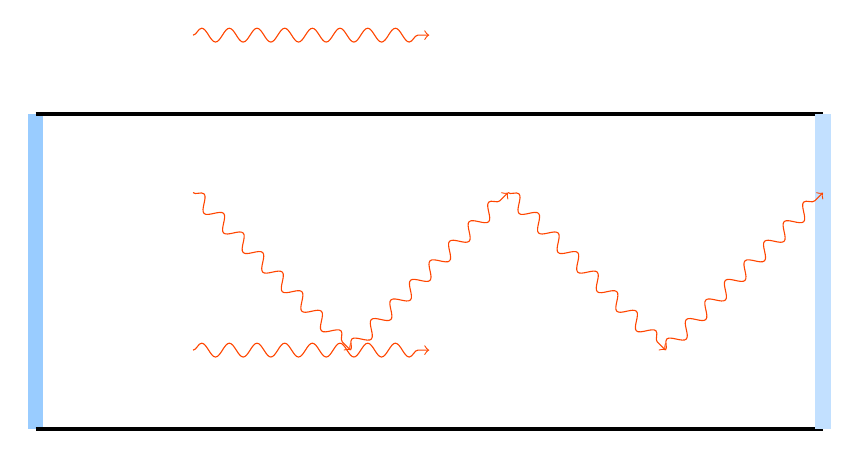
\begin{tikzpicture}

% Draw the left thick blue line
\draw[glass_blue, line width=2mm] (0,0) -- (0,-4);
% Draw the top thin black line
\draw[black, line width=0.5mm] (0,0) -- (10,0);
% Draw the bottom thin black line
\draw[black, line width=0.5mm] (0,-4) -- (10,-4);
% Draw the right thick blue line
\draw[glass_blue!60, line width=2mm] (10,0) -- (10,-4);

% Draw two parallel squiggly lines parallel to the black lines
\draw[->, snake it, atom_red] (2,1) -- (5,1);
\draw[->, snake it, atom_red] (2,-3) -- (5,-3);

% Draw two slanted squiggly lines hitting the blue lines with reflections
% First slanted line hitting the left blue line
\draw[->, snake it, atom_red] (2,-1) -- (4,-3);
\draw[->, snake it, atom_red] (4,-3) -- (6,-1);

% Second slanted line hitting the right blue line
\draw[->, snake it, atom_red] (6,-1) -- (8,-3);
\draw[->, snake it, atom_red] (8,-3) -- (10,-1);

\end{tikzpicture}
\end{document}
